\documentclass[usenames,dvipsnames]{beamer}
% \linespread{1.3}
\mode<presentation>{
\usetheme{Madrid}
\usecolortheme{default}
%\usecolortheme{beaver}
}
\usepackage{array}
\usepackage[utf8]{inputenc}
\usepackage{utopia}
\usepackage{verbatim}
\usepackage[portuguese]{babel}
\usepackage{pgfplots}
\pgfplotsset{/pgf/number format/use comma,compat=newest}
\usepackage{color}
\usepackage{amsmath,amsfonts,amssymb}
\usepackage{hyperref}
\usepackage{tikz}
\usepackage{proof}
\usepackage{caption}
\usepackage{soul}
%https://www.overleaf.com/project/61717826e515873b24296576
\usepackage{graphicx}
\usepackage{algorithm2e}
\usepackage{algorithmic}
\usepackage{xcolor}
% \usepackage{setspace}

\usetikzlibrary{positioning}

\setlength{\parskip}{1em}

%---------letters----------
\renewcommand{\AA}{\mathbb{A}}
\newcommand{\BB}{\mathbb{B}}
\newcommand{\CC}{\mathbb{C}}
\newcommand{\DD}{\mathbb{D}}
\newcommand{\EE}{\mathbb{E}}
\newcommand{\FF}{\mathbb{F}}
\newcommand{\GG}{\mathbb{G}}
\newcommand{\HH}{\mathbb{H}}
\newcommand{\II}{\mathbb{I}}
\newcommand{\JJ}{\mathbb{J}}
\newcommand{\KK}{\mathbb{K}}
\newcommand{\LL}{\mathbb{L}}
\newcommand{\MM}{\mathbb{M}}
\newcommand{\NN}{\mathbb{N}}
\newcommand{\OO}{\mathbb{O}}
\newcommand{\PP}{\mathbb{P}}
\newcommand{\QQ}{\mathbb{Q}}
\newcommand{\RR}{\mathbb{R}}
\renewcommand{\SS}{\mathbb{S}}
\newcommand{\TT}{\mathbb{T}}
\newcommand{\UU}{\mathbb{U}}
\newcommand{\VV}{\mathbb{V}}
\newcommand{\WW}{\mathbb{W}}
\newcommand{\XX}{\mathbb{X}}
\newcommand{\YY}{\mathbb{Y}}
\newcommand{\ZZ}{\mathbb{Z}}
% -----------
\newcommand{\cA}{\mathcal{A}}
\newcommand{\cB}{\mathcal{B}}
\newcommand{\cC}{\mathcal{C}}
\newcommand{\cD}{\mathcal{D}}
\newcommand{\cE}{\mathcal{E}}
\newcommand{\cF}{\mathcal{F}}
\newcommand{\cG}{\mathcal{G}}
\newcommand{\cH}{\mathcal{H}}
\newcommand{\cI}{\mathcal{I}}
\newcommand{\cJ}{\mathcal{J}}
\newcommand{\cK}{\mathcal{K}}
\newcommand{\cL}{\mathcal{L}}
\newcommand{\cM}{\mathcal{M}}
\newcommand{\cN}{\mathcal{N}}
\newcommand{\cO}{\mathcal{O}}
\newcommand{\cP}{\mathcal{P}}
\newcommand{\cQ}{\mathcal{Q}}
\newcommand{\cR}{\mathcal{R}}
\newcommand{\cS}{\mathcal{S}}
\newcommand{\cT}{\mathcal{T}}
\newcommand{\cU}{\mathcal{U}}
\newcommand{\cV}{\mathcal{V}}
\newcommand{\cW}{\mathcal{W}}
\newcommand{\cX}{\mathcal{X}}
\newcommand{\cY}{\mathcal{Y}}
\newcommand{\cZ}{\mathcal{Z}}



\newcommand\ldiaarg[1]{\langle#1\rangle}

\newcommand{\M}{\mathcal{M}}
% \newcommand{\LL}{\mathcal{L}} %for automata

\newcommand{\POL}{\mathsf{POL}}
\newcommand{\EPL}{\mathsf{EPL}}
\newcommand{\Decide}{\mathsf{Decide}}
\newcommand{\DecidePSPACE}{\mathsf{mcPOL}}
\newcommand{\reach}{\mathsf{PSPACEReach}}
\newcommand{\CreateDelta}{\mathsf{CreateDelta}}
\newcommand{\StringRepresent}{\mathsf{StringRepresent}}
\newcommand{\StoreStrings}{\mathsf{StoreStrings}}
\newcommand{\ResidueByLetter}{\mathsf{ResidueByLetter}}
\newcommand{\ResidueByWord}{\mathsf{ResidueByWord}}
\newcommand{\AuxOut}{\mathsf{AuxOut}}
\newcommand{\GetSetNP}{\mathsf{GetSetNP}}
\newcommand{\T}{\mathsf{True}}
\newcommand{\Fa}{\mathsf{False}}
\newcommand{\tr}{\mathsf{tr}}
\newcommand{\starfree}{\mathsf{Star\mbox{-}Free}}
\newcommand{\word}{\mathsf{Word}}
\newcommand{\existential}{\mathsf{Existential}}
\newcommand{\PSPACE}{\mathsf{PSPACE}}
\newcommand{\NPSPACE}{\mathsf{NPSPACE}}
\newcommand{\PTime}{\mathsf{P}}
\newcommand{\NP}{\mathsf{NP}}
\newcommand{\EXPTime}{\mathsf{EXPTIME}}
\newcommand{\NEXPTime}{\mathsf{NEXPTIME}}
\newcommand{\PTIME}{\mathsf{PTIME}}
\newcommand{\automaton}{\mathcal A}
\newcommand{\modelM}{\mathcal M}
\newcommand{\languageof}[1]{L({#1})}
\newcommand{\set}[1]{\{#1\}}
\newcommand{\suchthat}{\mid}
\newcommand{\union}{\cup}
\newcommand{\Union}{\bigcup}
\newcommand{\ep}{\ensuremath{\varepsilon}}

\newcommand{\obsright}{\blacktriangleright}
\newcommand{\obsleft}{\blacktriangleleft}
\newcommand{\obsup}{\blacktriangle}
\newcommand{\obsdown}{\blacktriangledown}

\newcommand{\expwater}{(\obsright \union \obsup)^* (\obsdown \union \obsleft \union \ep) (\obsright \union \obsup)^*}
\newcommand{\exppower}{(\obsleft \union \obsdown)^* (\obsup \union \obsright \union \ep) (\obsleft \union \obsdown)^*}
\newcommand{\exppatrol}{(\obsright^+ \obsdown^+ \obsleft^+ \obsup^+)^*}

\newcommand\drone{
\includegraphics[height=3ex]{images/E1D2_color.png}}
\newcommand\agentA{
\includegraphics[height=3ex]{images/agent A icon.png}}
\newcommand\agentB{
\includegraphics[height=3ex]{images/agent b icon.png}}
\newcommand\water{
\includegraphics[height=3ex]{images/1F4A7_color.png}}

\newcommand\algoaccept{\textbf{accept}}
\newcommand\algoreject{\textbf{reject}}
\newcommand{\regdiv}[1]{\ensuremath{\backslash} #1}

\renewcommand{\phi}{\varphi}

% tiling macros

%\tile x y colorleft colorup colorright colorbottom
\newcommand{\tile}[6]{
	%left
	\draw[fill=#3] (#1,#2) -- (#1,#2+1) -- (#1+0.5, #2+0.5) -- (#1, #2);
	%
	%up
	\draw[fill=#4] (#1,#2+1)-- (#1+1,#2+1) -- (#1 +0.5, #2+0.5) -- (#1, #2+1);
	%
	%right
	\draw[fill=#5] (#1+1,#2)-- (#1+1,#2+1) -- (#1 +0.5, #2+0.5) -- (#1 +1, #2);
	%
	%bottom
	\draw[fill=#6] (#1,#2)-- (#1 +1,#2) -- (#1 +0.5, #2+0.5) -- (#1, #2);
	%
	\draw[fill=black] (#1+0.5, #2+0.5) -- (#1+0.6, #2+0.4) -- (#1+0.4, #2+0.4) -- cycle;
}


\newcommand{\tilewc}[4]{\tikz{\tile{0}{0}{#1}{#2}{#3}{#4}}}
\newcommand{\tilewcsmall}[4]{\tikz[scale=0.5]{\tile{0}{0}{#1}{#2}{#3}{#4}}}


\newcommand{\tiletextcolorwc}[4]{\raisebox{-5mm}{\scalebox{0.7}{\tikz[scale=1.5]{\tiletextcolor{0}{0}{#1}{#2}{#3}{#4}}}}}




\newcommand{\tiletextwc}[4]{\raisebox{-5mm}{\scalebox{0.5}{\tikz[scale=1.5]{\tiletext{0}{0}{#1}{#2}{#3}{#4}}}}}
\newcommand{\tiletextwcsmall}[4]{\raisebox{-2mm}{\scalebox{0.5}{\tikz[scale=1]{\tiletext{0}{0}{#1}{#2}{#3}{#4}}}}}
\newcommand{\tiletextwcbig}[4]{\tikz[scale=2]{\tiletext{0}{0}{#1}{#2}{#3}{#4}}}

\newcommand{\tiletext}[6]{
	\tile {#1} {#2} {none} {none} {none} {none}
	\node at (#1+0.25, #2+0.5) {#3}; %left
	\node at (#1+0.5, #2+0.8) {#4}; %up
	\node at (#1+0.75, #2+0.5) {#5}; %right
	\node at (#1+0.5, #2+0.1) {#6}; %bottom
}




\newcommand{\tilered}{red!80}
\newcommand{\tileyellow}{yellow!50}
\newcommand{\tilegreen}{green!70}
\newcommand{\tileblue}{blue!50}
\newcommand{\tilewhite}{white}

\newcommand{\whitetile}[2]{\tile{#1}{#2}{white}{white}{white}{white}}

\newcommand{\anytile}{t}
\newcommand{\tileseed}{t_0}
\newcommand{\tileset}{T}


\tikzstyle{rectNode} = [rectangle, text centered]
\tikzstyle{fastate} = [circle, text centered, draw = black]
\tikzstyle{dots} = [circle, draw = black, fill = black, inner sep=1pt]

\tikzstyle{world} = [draw]
\tikzstyle{worldwhite} = [draw = white]
\tikzstyle{tape} = [draw,thick,minimum width=1,minimum height=1]

\makeatletter
\let\HL\hl
\renewcommand\hl{%
  \let\set@color\beamerorig@set@color
  \let\reset@color\beamerorig@reset@color
  \HL}
\makeatother



\title[]{Logic and Complexity}
\author[]{
\textbf{Avijeet Ghosh}\inst{1}}
\institute[Indian Statistical Institute, Kolkata]{\inst{1} Indian Statistical Institute, Kolkata}
\date[September 2024]

\AtBeginSection[]
{
\begin{frame}{Table of Contents}
\tableofcontents[currentsection]
\end{frame}
}


\begin{document}

\begin{frame}
 \maketitle
\end{frame}
% \begin{frame}{Table of Contents}
%     \tableofcontents
% \end{frame}

% \section{Theory of Computation}
\begin{frame}{A System of Proofs}
    \begin{columns}
        \begin{column}{0.3\textwidth}
            \begin{tikzpicture}
                \node (h) at (0,0) {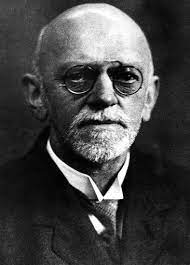
\includegraphics[width = 2cm]{images/hilbert.jpeg}};
                \node (q) at (2,0) {
\includegraphics[width = 2cm]{images/question.jpg}};
            \end{tikzpicture}
        \end{column}
        \begin{column}{0.7\textwidth}
            \begin{itemize}
                \item<1-> A Formal System of Mathematical Proofs
                \begin{itemize}
                    \item<2-> Axioms $\cA = \{A_1, A_2,\ldots, A_k\}$
                    \item<3-> Truth-preserving rules $\cI = \{I_1,\ldots, I_m\}$
                            \[
                                I_i = \infer{C}{%
                                            S_1,
                                            S_2,\ldots,
                                            S_n
                                        }
                            \] 
                \end{itemize}
                \item<4-> Objective: Anything true has a proof

                \begin{tikzpicture}[scale=0.8, transform shape]
                    \node (ai) at (0,0) {$A_i$};
                    \node (aj) at (1,0) {$A_j$};
                    \node (ak) at (2,0) {$A_k$};
                    \node (al) at (3,0) {$A_\ell$};
                    \node (t1) at (0.5,1) {$T_1$};
                    \node (t2) at (2.5,1) {$T_2$};
                    \node (t) at (1.5,2) {$T$};

                    \draw[->] (ai) edge node[left]{$I_{i'}$} (t1);
                    \draw[->] (aj) edge (t1);
                    \draw[->] (ak) edge (t2);
                    \draw[->] (al) edge node[right]{$I_{j'}$} (t2);
                    \draw[->] (t1) edge node[left]{$I_{k'}$} (t);
                    \draw[->] (t2) edge (t);
                \end{tikzpicture}
            \end{itemize}
        \end{column}
    \end{columns}
\end{frame}
\begin{frame}{Hilbert's Questions}
    \begin{tikzpicture}
        \node (h) at (0,0) {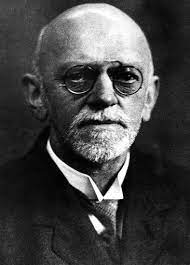
\includegraphics[width = 1cm]{images/hilbert.jpeg}};
        \node (q1) at (5,3) {$1.$};
        \node (q2) at (5,0) {$2.$};
        \node (q3) at (5,-3) {$3.$};
        \draw[->] (h) edge node[above]{\Large ?} (q1);
        \draw[->] (h) edge node[above]{\Large ?} (q2);
        \draw[->] (h) edge node[above]{\Large ?} (q3);\pause 

        \node (q1q) at (6,3) {Complete};
        \node (q2q) at (6,0) {Consistent};
        \node (q1q) at (6,-3) {Decidable};\pause

        \node (q1dec) at (7,3) {\textcolor{red}{\Large X}};
        \node (q1god) at (8,3) {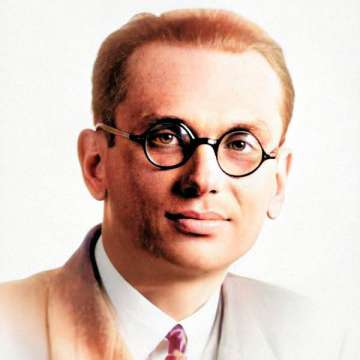
\includegraphics[width = 1cm]{images/godel.jpg}};
        \node (q1state) at (7.5,2) {Some Truths cannot be proven};\pause

        \node (q2dec) at (7,0) {\textcolor{Fuchsia}{\Large ?}};
        \node (q2god) at (8,0) {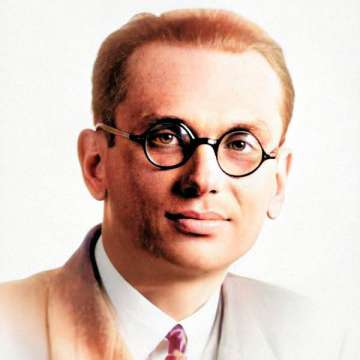
\includegraphics[width = 1cm]{images/godel.jpg}};
        \node (q2state) at (7.5,-1) {Proving its own consistency beyond system};\pause

        \node (q3dec) at (7.3,-3) {
\includegraphics[width = 1cm]{images/wonder.jpg}};
        \node (q3talk) at (8.3,-3) {This talk};
        \node (q3state) at (7.5,-4) {Given a statement and axioms, is there a proof?};
    \end{tikzpicture}
\end{frame}

\begin{frame}{Computability}
    \begin{itemize}
        \item<1-> \textbf{NEED:} Given $S$ and $\cA$, "procedure" to decide whether there is a proof
        \begin{itemize}
            \item<2-> For any axiom system $(\cA,\cI)$ and any statement $S$
            $ f(S,\cA,\cI) = 
            \begin{cases} 
                1 & \cA\vdash_\cI S \\
                0 & \cA\nvdash_\cI S  
            \end{cases}
            $
            \item<3-> Is $f$ \emph{computable}?
        \end{itemize}
        \item<4-> What is \emph{computability}?
        \item<5-> \textbf{Example 1}: $\forall x\in\NN, f(x) = x^2 + 2x + 1$
        \begin{itemize}
            \item<6-> $f(13) = ?$
        \end{itemize}
        \item<7-> \textbf{Example 2}: $\forall x\in\NN,\forall y\in\NN f(x,y) = x^y + xy + 1$
        \begin{itemize}
            \item<8-> $f(13,12) = ?$
            \item<9-> \bf HARDER
        \end{itemize}
    \end{itemize}
\end{frame}

\begin{frame}{Computability}
    \begin{itemize}
        \item<1-> Proper Tiling:
        \begin{itemize}
            \item<2-> Given a set of tiles $\cT$
            \item[]<2->
            \begin{tikzpicture}[scale=0.5]
            \node[text width=2cm] at (-2, 1.5) 
            {					
                \tilewcsmall \tilewhite \tilewhite \tilegreen\tilered
                
                \tilewcsmall \tilegreen\tilewhite\tilegreen\tilered
                
                \tilewcsmall \tilegreen\tilewhite\tilewhite\tilewhite
                
                \tilewcsmall \tilewhite \tilered\tilewhite\tilered
            };
            
            \node[text width=2cm] at (-0.5, 1.5) {
                \tilewcsmall \tilegreen \tilewhite\tilegreen\tilewhite
                
                \tilewcsmall \tilewhite \tilewhite\tilewhite\tilegreen
                
                \tilewcsmall \tilewhite\tilered\tilegreen\tilewhite
                
                \tilewcsmall \tilegreen\tilered\tilered\tilewhite
                
                \tilewcsmall \tilered	\tilegreen\tilewhite\tilewhite
                
            };
            \end{tikzpicture}
            \item<3-> A Proper tiling on a finite grid:
            \item[]<3-> \begin{tikzpicture}[scale=0.5, baseline=-15mm]
                % posx posy left up right down
                      \tile 0 1 \tilewhite \tilewhite \tilegreen\tilewhite
                      \tile 1 1 \tilegreen\tilewhite\tilegreen\tilewhite
                      \tile 2 1 \tilegreen\tilewhite\tilegreen\tilewhite
                      \tile 3 1 \tilegreen\tilewhite\tilered\tilered
                      \tile 0 0 \tilewhite \tilewhite \tilegreen\tilered
                      \tile 1 0 \tilegreen\tilewhite\tilegreen\tilered
                      \tile 2 0 \tilegreen\tilewhite\tilewhite\tilewhite
                      \tile 3 0 \tilewhite\tilered\tilewhite\tilered
                      \tile 0 {-1} \tilewhite \tilered\tilewhite\tilered
                      \tile 1 {-1} \tilewhite \tilered\tilewhite\tilered
                      \tile 2 {-1} \tilewhite \tilewhite\tilewhite\tilegreen
                      \tile 3 {-1} \tilewhite\tilered\tilewhite\tilered
                      \tile 0 {-2} \tilewhite\tilered\tilegreen\tilewhite
                      \tile 1 {-2} \tilegreen\tilered\tilered\tilewhite
                      \tile 2 {-2} \tilered	\tilegreen\tilewhite\tilewhite
                      \tile 3 {-2} \tilewhite\tilered\tilewhite\tilered
                      \end{tikzpicture}
        \end{itemize} 
        \item<4-> $ f(\cT) = 
            \begin{cases} 
                1 & \mbox{Proper tiling covering infinite grid} \\
                0 & \mbox{No such proper tiling}  
            \end{cases}
            $
    \end{itemize}
\end{frame}

\begin{frame}{Model of Computability}
    \begin{itemize}
        \item<1-> $f(x) = x^2 + 2x +1$. 
        \item<2-> $f(13) = 13^2 + (2x13) + 1$
        \item<3-> Local rules:
                \begin{itemize}
                    \item<4-> Rule of multiplication
                    \item<5-> Rule of addition
                \end{itemize} 
        \item<6-> Local states:
                \begin{enumerate}
                    \item<7-> Initial $13^2 + (2x13) + 1$
                    \item<8-> All multiplication done $169 + 26 + 1$
                    \item<9-> All addition done $196$
                    \item<10-> Final value $196$
                \end{enumerate}
        \item<11-> \textbf{NEED: MODEL} Anything that model can compute is computable
        \item<12-> Turing Machine, Lambda Calculus 
    \end{itemize}
\end{frame}

\begin{frame}{The Turing Machine}
    \begin{tikzpicture}
        \node[tape] (t1) at (4,1)  {$0$};
        \node[tape] (t2) at (4.5,1)  {$1$};
        \node[tape] (t3) at (5,1)  {$0$};
        \node[tape] (t4) at (5.5,1)  {$0$};
        \node[tape] (t5) at (6,1)  {$1$};
        \node[tape] (t6) at (6.5,1)  {$0$};
        \node[tape] (t7) at (7,1)  {$0$};
        \node[tape] (t8) at (7.5,1)  {$0$};
        \node[tape] (t9) at (8,1)  {$0$};
        \node (d) at (9,1) {$\ldots\ldots$};
        \node (d2) at (3,1) {$\ldots\ldots$};\pause
        \node[align = center, rectangle, draw] (M) at (4.5,-3) 
        {\begin{tikzpicture}
                \node (s) at (0,0) {\Large \textbf{$q_0$}};\pause
                \node[align = center, circle, draw, very thick] (q0) at (0,-2) {\textbf{$q_0$}};
                \node[align = center, circle, draw] (q1) at (3,-2) {$q_1$};
                \node[align = center, circle, draw] (q3) at (0,-5) {$q_3$};

                \draw[->, very thick] (q0) edge node[above]{\small $0:1,R$} (q1);
                \draw[->] (q0) edge node[left]{\small $1:0,R$} (q3);
                \draw[->] (q1) .. controls (2,-4.5) .. node[below]{\small $~~~~~~0:1,L$} (q3);
                \draw[->] (q1) edge [loop above] node{\small $1:0,R$} (q1);
                \draw[->] (q3) edge node[above]{\small $1:1,R~~~~~~~$} (q1);
                \draw[->] (q3) edge [loop left] node{\small $0:0,R$} (q3);

        \end{tikzpicture}};
        \draw[->] (M) edge (t1);
    \end{tikzpicture}
\end{frame}

\begin{frame}{The Turing Machine}
    \begin{tikzpicture}
        \node[tape] (t1) at (4,1)  {$0$};
        \node[tape] (t2) at (4.5,1)  {$1$};
        \node[tape] (t3) at (5,1)  {$0$};
        \node[tape] (t4) at (5.5,1)  {$0$};
        \node[tape] (t5) at (6,1)  {$1$};
        \node[tape] (t6) at (6.5,1)  {$0$};
        \node[tape] (t7) at (7,1)  {$0$};
        \node[tape] (t8) at (7.5,1)  {$0$};
        \node[tape] (t9) at (8,1)  {$0$};
        \node (d) at (9,1) {$\ldots\ldots$};
        \node (d2) at (3,1) {$\ldots\ldots$};
        \node[align = center, rectangle, draw] (M) at (4.5,-3) 
        {\begin{tikzpicture}
                \node (s) at (0,0) {\Large \textbf{$q_0$}};
                \node[align = center, circle, draw, very thick] (q0) at (0,-2) {\textbf{$q_0$}};
                \node[align = center, circle, draw] (q1) at (3,-2) {$q_1$};
                \node[align = center, circle, draw] (q3) at (0,-5) {$q_3$};

                \draw[->, very thick] (q0) edge node[above]{\small $0:1,R$} (q1);
                \draw[->] (q0) edge node[left]{\small $1:0,R$} (q3);
                \draw[->] (q1) .. controls (2,-4.5) .. node[below]{\small $~~~~~~0:1,L$} (q3);
                \draw[->] (q1) edge [loop above] node{\small $1:0,R$} (q1);
                \draw[->] (q3) edge node[above]{\small $1:1,R~~~~~~~$} (q1);
                \draw[->] (q3) edge [loop left] node{\small $0:0,R$} (q3);

        \end{tikzpicture}};
        \draw[->] (M) edge (t1);
    \end{tikzpicture}
\end{frame}
\begin{frame}{The Turing Machine}
    \begin{tikzpicture}
        \node[tape] (t1) at (4,1)  {$1$};
        \node[tape] (t2) at (4.5,1)  {$1$};
        \node[tape] (t3) at (5,1)  {$0$};
        \node[tape] (t4) at (5.5,1)  {$0$};
        \node[tape] (t5) at (6,1)  {$1$};
        \node[tape] (t6) at (6.5,1)  {$0$};
        \node[tape] (t7) at (7,1)  {$0$};
        \node[tape] (t8) at (7.5,1)  {$0$};
        \node[tape] (t9) at (8,1)  {$0$};
        \node (d) at (9,1) {$\ldots\ldots$};
        \node (d2) at (3,1) {$\ldots\ldots$};
        \node[align = center, rectangle, draw] (M) at (4.5,-3) 
        {\begin{tikzpicture}
                \node (s) at (0,0) {\Large \textbf{$q_1$}};
                \node[align = center, circle, draw] (q0) at (0,-2) {\textbf{$q_0$}};
                \node[align = center, circle, draw, very thick] (q1) at (3,-2) {$q_1$};
                \node[align = center, circle, draw] (q3) at (0,-5) {$q_3$};

                \draw[->] (q0) edge node[above]{\small $0:1,R$} (q1);
                \draw[->] (q0) edge node[left]{\small $1:0,R$} (q3);
                \draw[->] (q1) .. controls (2,-4.5) .. node[below]{\small $~~~~~~0:1,L$} (q3);
                \draw[->, very thick] (q1) edge [loop above] node{\small $1:0,R$} (q1);
                \draw[->] (q3) edge node[above]{\small $1:1,R~~~~~~~$} (q1);
                \draw[->] (q3) edge [loop left] node{\small $0:0,R$} (q3);

        \end{tikzpicture}};
        \draw[->] (M) edge (t2);
    \end{tikzpicture}
\end{frame}
\begin{frame}{The Turing Machine}
    \begin{tikzpicture}
        \node[tape] (t1) at (4,1)  {$1$};
        \node[tape] (t2) at (4.5,1)  {$0$};
        \node[tape] (t3) at (5,1)  {$0$};
        \node[tape] (t4) at (5.5,1)  {$0$};
        \node[tape] (t5) at (6,1)  {$1$};
        \node[tape] (t6) at (6.5,1)  {$0$};
        \node[tape] (t7) at (7,1)  {$0$};
        \node[tape] (t8) at (7.5,1)  {$0$};
        \node[tape] (t9) at (8,1)  {$0$};
        \node (d) at (9,1) {$\ldots\ldots$};
        \node (d2) at (3,1) {$\ldots\ldots$};
        \node[align = center, rectangle, draw] (M) at (4.5,-3) 
        {\begin{tikzpicture}
                \node (s) at (0,0) {\Large \textbf{$q_1$}};
                \node[align = center, circle, draw] (q0) at (0,-2) {\textbf{$q_0$}};
                \node[align = center, circle, draw, very thick] (q1) at (3,-2) {$q_1$};
                \node[align = center, circle, draw] (q3) at (0,-5) {$q_3$};

                \draw[->] (q0) edge node[above]{\small $0:1,R$} (q1);
                \draw[->] (q0) edge node[left]{\small $1:0,R$} (q3);
                \draw[->, very thick] (q1) .. controls (2,-4.5) .. node[below]{\small $~~~~~~0:1,L$} (q3);
                \draw[->] (q1) edge [loop above] node{\small $1:0,R$} (q1);
                \draw[->] (q3) edge node[above]{\small $1:1,R~~~~~~~$} (q1);
                \draw[->] (q3) edge [loop left] node{\small $0:0,R$} (q3);

        \end{tikzpicture}};
        \draw[->] (M) edge (t3);
    \end{tikzpicture}
\end{frame}
\begin{frame}{The Turing Machine}
    \begin{tikzpicture}
        \node[tape] (t1) at (4,1)  {$1$};
        \node[tape] (t2) at (4.5,1)  {$0$};
        \node[tape] (t3) at (5,1)  {$1$};
        \node[tape] (t4) at (5.5,1)  {$0$};
        \node[tape] (t5) at (6,1)  {$1$};
        \node[tape] (t6) at (6.5,1)  {$0$};
        \node[tape] (t7) at (7,1)  {$0$};
        \node[tape] (t8) at (7.5,1)  {$0$};
        \node[tape] (t9) at (8,1)  {$0$};
        \node (d) at (9,1) {$\ldots\ldots$};
        \node (d2) at (3,1) {$\ldots\ldots$};
        \node[align = center, rectangle, draw] (M) at (4.5,-3) 
        {\begin{tikzpicture}
                \node (s) at (0,0) {\Large \textbf{$q_3$}};
                \node[align = center, circle, draw] (q0) at (0,-2) {\textbf{$q_0$}};
                \node[align = center, circle, draw] (q1) at (3,-2) {$q_1$};
                \node[align = center, circle, draw, very thick] (q3) at (0,-5) {$q_3$};

                \draw[->] (q0) edge node[above]{\small $0:1,R$} (q1);
                \draw[->] (q0) edge node[left]{\small $1:0,R$} (q3);
                \draw[->] (q1) .. controls (2,-4.5) .. node[below]{\small $~~~~~~0:1,L$} (q3);
                \draw[->] (q1) edge [loop above] node{\small $1:0,R$} (q1);
                \draw[->] (q3) edge node[above]{\small $1:1,R~~~~~~~$} (q1);
                \draw[->, very thick] (q3) edge [loop left] node{\small $0:0,R$} (q3);

        \end{tikzpicture}};
        \draw[->] (M) edge (t2);
    \end{tikzpicture}
\end{frame}
\begin{frame}{The Turing Machine}
    \begin{tikzpicture}
        \node[tape] (t1) at (4,1)  {$1$};
        \node[tape] (t2) at (4.5,1)  {$0$};
        \node[tape] (t3) at (5,1)  {$1$};
        \node[tape] (t4) at (5.5,1)  {$0$};
        \node[tape] (t5) at (6,1)  {$1$};
        \node[tape] (t6) at (6.5,1)  {$0$};
        \node[tape] (t7) at (7,1)  {$0$};
        \node[tape] (t8) at (7.5,1)  {$0$};
        \node[tape] (t9) at (8,1)  {$0$};
        \node (d) at (9,1) {$\ldots\ldots$};
        \node (d2) at (3,1) {$\ldots\ldots$};
        \node[align = center, rectangle, draw] (M) at (4.5,-3) 
        {\begin{tikzpicture}
                \node (s) at (0,0) {\Large \textbf{$q_3$}};
                \node[align = center, circle, draw] (q0) at (0,-2) {\textbf{$q_0$}};
                \node[align = center, circle, draw] (q1) at (3,-2) {$q_1$};
                \node[align = center, circle, draw, very thick] (q3) at (0,-5) {$q_3$};

                \draw[->] (q0) edge node[above]{\small $0:1,R$} (q1);
                \draw[->] (q0) edge node[left]{\small $1:0,R$} (q3);
                \draw[->] (q1) .. controls (2,-4.5) .. node[below]{\small $~~~~~~0:1,L$} (q3);
                \draw[->] (q1) edge [loop above] node{\small $1:0,R$} (q1);
                \draw[->, very thick] (q3) edge node[above]{\small $1:1,R~~~~~~~$} (q1);
                \draw[->] (q3) edge [loop left] node{\small $0:0,R$} (q3);

        \end{tikzpicture}};
        \draw[->] (M) edge (t3);
    \end{tikzpicture}
\end{frame}
\begin{frame}{The Turing Machine}
    \begin{tikzpicture}
        \node[tape] (t1) at (4,1)  {$0$};
        \node[tape] (t2) at (4.5,1)  {$1$};
        \node[tape] (t3) at (5,1)  {$0$};
        \node[tape] (t4) at (5.5,1)  {$0$};
        \node[tape] (t5) at (6,1)  {$1$};
        \node[tape] (t6) at (6.5,1)  {$0$};
        \node[tape] (t7) at (7,1)  {$0$};
        \node[tape] (t8) at (7.5,1)  {$0$};
        \node[tape] (t9) at (8,1)  {$0$};
        \node (d) at (9,1) {$\ldots\ldots$};
        \node (d2) at (3,1) {$\ldots\ldots$};
        \node[align = center, rectangle, draw] (M) at (4.5,-3) 
        {\begin{tikzpicture}
                \node (s) at (0,0) {\Large \textbf{$q_1$}};
                \node[align = center, circle, draw] (q0) at (0,-2) {\textbf{$q_0$}};
                \node[align = center, circle, draw, very thick] (q1) at (3,-2) {$q_1$};
                \node[align = center, circle, draw] (q3) at (0,-5) {$q_3$};

                \draw[->] (q0) edge node[above]{\small $0:1,R$} (q1);
                \draw[->] (q0) edge node[left]{\small $1:0,R$} (q3);
                \draw[->, very thick] (q1) .. controls (2,-4.5) .. node[below]{\small $~~~~~~0:1,L$} (q3);
                \draw[->] (q1) edge [loop above] node{\small $1:0,R$} (q1);
                \draw[->] (q3) edge node[above]{\small $1:1,R~~~~~~~$} (q1);
                \draw[->] (q3) edge [loop left] node{\small $0:0,R$} (q3);

        \end{tikzpicture}};
        \draw[->] (M) edge (t4);
    \end{tikzpicture}
\end{frame}

\begin{frame}{The Turing Machine}
    \begin{columns}
        \begin{column}{0.3\textwidth}
            \begin{tikzpicture}
                \node (turing) at (0,0) {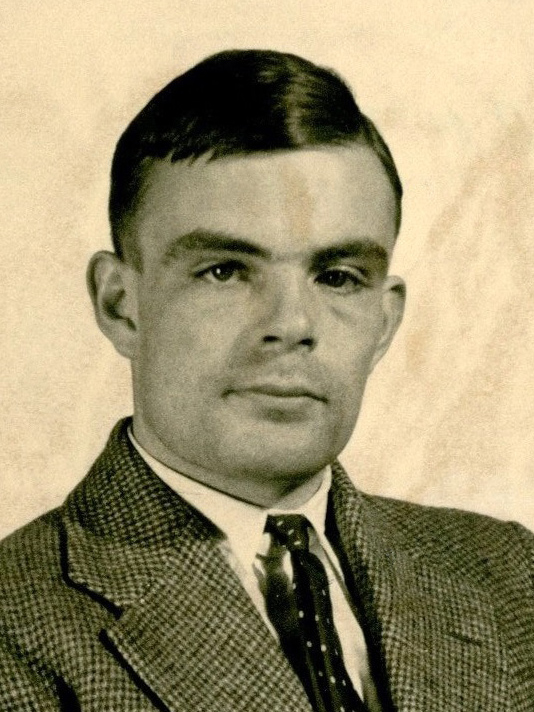
\includegraphics[width = 3cm]{images/turing.jpg}}; 
            \end{tikzpicture}
        \end{column}
        \begin{column}{0.7\textwidth}
            \begin{itemize}
                \item $\cM = \ldiaarg{Q,q_0\in Q, \Sigma, \delta, F\subseteq Q}$
                    \begin{itemize}
                        \item $Q$: finite set of states
                        \item $\Sigma$: alphabet
                        \item $\delta:Q\times\Sigma\rightarrow Q\times\Sigma\cup\{R,L\}$ transition rule
                    \end{itemize}
                \item Decision functions:~$f(x\in\{0,1\}^\star)\in\{0,1\}$
                \item \textbf{Other MODELS}: Church's Lambda Calculus
                \item[]
                
                \begin{block}{Church-Turing Thesis}
                    Any computable function can be computed by a Turing Machine/$\lambda$-Calculus.
                \end{block}

            \end{itemize}
        \end{column}
    \end{columns}
\end{frame}

\begin{frame}{Complexity Theory}
    \begin{itemize}
        \item<1-> \textbf{Model:} Turing Machine (TM)
        \item<2-> Bounding resource usage of computation wrt input size $n$
            \begin{itemize}
                \item<3-> \textbf{Time}: Steps a TM takes
                \item<4-> \textbf{Space}: Tape space used
                \item<5-> \textbf{Asymptotical}: $2\cC(n) + 3\equiv 55\cC(n) + 7$\\
                ~~~~~~~~~~~~~~~~~~~~$2^{\cC(n)}\not\equiv 3^{\cC(n)}$
            \end{itemize}
        \item<6-> Difficulty between classes of problems (Decision functions)
        \item<7-> Decision functions gives Language
        \begin{itemize}
            \item<8-> Language of $f$ $\cL_f\subseteq\Sigma^\star$
            \item<9-> $f(x) = 1$ $\equiv$ $\cM_f(x)$ accepts $\equiv$ $x\in \cL_f$
        \end{itemize}
    \end{itemize}
\end{frame}

\begin{frame}{Polynomial Complexity}
    Consider the following problems:
    \begin{itemize}
        \item<1-> Given a tuple of $n$ integers, \textbf{are they SORTED}?
        \begin{itemize}
            \item<2-> $\ldiaarg{23,45,79,127}$
            \item<3-> Easily solvable
            \item<4-> Compare adjascent pair (constant steps $c$)
            \item<5-> Check for all adjascent pairs ($\leq n$)
            \item<6-> Total steps $\sim cn$
        \end{itemize}
        \item<7-> Given a propositional formula $\varphi$, \textbf{is it SATISFIABLE}?
        \begin{itemize}
            \item<8-> $\varphi = (x_1\vee \neg x_2)\wedge (x_2\vee \neg x_3\vee \neg x_1)\wedge (x_3\vee x_1\vee x_2)$
            \item<9-> Harder to solve
            \item<10-> If \textbf{SATISFIABLE}, what is the certificate?
            \item<11-> How big?
            \item<12-> If certificate given, how much time to verify?
        \end{itemize}
    \end{itemize}
\end{frame}

\begin{frame}{Non-determinism}
    \begin{itemize}
        \item $\varphi = (x_1\vee \neg x_2)\wedge (x_2\vee \neg x_3\vee \neg x_1)\wedge (x_3\vee x_1\vee x_2)$
        \item TM steps:
        \item[] 
        \begin{tikzpicture}
            \node (x1) at (0,0){$x_1$};
            \node (x2l) at (-2,-1){$x_2$};
            \node (x2r) at (2,-1){$x_2$};
            \node (x3rr) at (3,-2){$x_3$};
            \node (x3rl) at (1,-2){$x_3$};
            \node (x3lr) at (-1,-2){$x_3$};
            \node (x3ll) at (-3,-2){$x_3$};
            \node (000) at (-3.5,-3){\textcolor{red}{X}};
            \node (001) at (-2.5,-3){\textcolor{green}{\checkmark}};
            \node (010) at (-1.5,-3){\textcolor{red}{X}};
            \node (011) at (-0.5,-3){\textcolor{red}{X}};
            \node (100) at (0.5,-3){\textcolor{green}{\checkmark}};
            \node (101) at (1.5,-3){\textcolor{red}{X}};
            \node (110) at (2.5,-3){\textcolor{green}{\checkmark}};
            \node (111) at (3.5,-3){\textcolor{green}{\checkmark}};


            \draw[->] (x1) edge[dotted] (x2l);
            \draw[->] (x1) edge (x2r);
            \draw[->] (x2l) edge[dotted] (x3ll);
            \draw[->] (x2l) edge (x3lr);
            \draw[->] (x2r) edge[dotted] (x3rl);
            \draw[->] (x2r) edge (x3rr);
            
            \draw[->] (x3ll) edge[dotted] (000);
            \draw[->] (x3lr) edge[dotted] (010);
            \draw[->] (x3rl) edge[dotted] (100);
            \draw[->] (x3rr) edge[dotted] (110);

            \draw[->] (x3ll) edge (001);
            \draw[->] (x3lr) edge (011);
            \draw[->] (x3rl) edge (101);
            \draw[->] (x3rr) edge (111);
        \end{tikzpicture}
    \end{itemize}
\end{frame}

\begin{frame}{Non-determinism}
    \begin{itemize}
        \item $\varphi = (x_1\vee \neg x_2)\wedge (x_2\vee \neg x_3\vee \neg x_1)\wedge (x_3\vee x_1\vee x_2)$
        \item Lucky TM steps:
        \item[] 
        \begin{tikzpicture}
            \node (x1) at (0,0){$x_1$};
            \node (x2l) at (-2,-1){$x_2$};
            \node (x2r) at (2,-1){$x_2$};
            \node (x3rr) at (3,-2){$x_3$};
            \node (x3rl) at (1,-2){$x_3$};
            \node (x3lr) at (-1,-2){$x_3$};
            \node (x3ll) at (-3,-2){$x_3$};
            \node (000) at (-3.5,-3){\textcolor{red}{X}};
            \node (001) at (-2.5,-3){\textcolor{green}{\checkmark}};
            \node (010) at (-1.5,-3){\textcolor{red}{X}};
            \node (011) at (-0.5,-3){\textcolor{red}{X}};
            \node (100) at (0.5,-3){\textcolor{green}{\checkmark}};
            \node (101) at (1.5,-3){\textcolor{red}{X}};
            \node (110) at (2.5,-3){\textcolor{green}{\checkmark}};
            \node (111) at (3.5,-3){\textcolor{green}{\checkmark}};


            \draw[->] (x1) edge[dotted] (x2l);
            \draw[->] (x1) edge (x2r);
            \draw[->] (x2l) edge[dotted] (x3ll);
            \draw[->] (x2l) edge (x3lr);
            \draw[->] (x2r) edge[dotted] (x3rl);
            \draw[->] (x2r) edge (x3rr);
            
            \draw[->] (x3ll) edge[dotted] (000);
            \draw[->] (x3lr) edge[dotted] (010);
            \draw[->] (x3rl) edge[dotted] (100);
            \draw[->] (x3rr) edge[dotted] (110);

            \draw[->] (x3ll) edge (001);
            \draw[->] (x3lr) edge (011);
            \draw[->] (x3rl) edge (101);
            \draw[->] (x3rr) edge (111);
            \pause
            \draw[->] (x1) edge[dotted, red, very thick] (x2l);\pause
            \draw[->] (x2l) edge[dotted, red, very thick] (x3ll);\pause
            \draw[->] (x3ll) edge[red, very thick] (001);
        \end{tikzpicture}
        \item This Lucky TM is \emph{quick} iff small certificate, quick verify
        \item This Lucky TM is called \textbf{Non-deterministic}
    \end{itemize}
\end{frame}

\begin{frame}{Complexity Classes}
    \begin{itemize}
        \item $\cL\in\PTime$:= Steps$(\cM_\cL(x))\leq O(|x|^c)$ 
        \item $\cL\in\NP$:= Steps$(\cM_\cL(x))\leq O(|x|^c)$, $\cM_\cL$ is Non-deterministic
        \item $\PTime\subset_?\NP$
        \item $\cL\in\EXPTime$:= Steps$(\cM_\cL(x))\leq O(2^{|x|^c})$
        \item $\cL\in\NEXPTime$:= Steps$(\cM_\cL(x))\leq O(2^{|x|^c})$, $\cM_\cL$ is ND
        \item $\PTime\subseteq_?\NP\subseteq_?\EXPTime\subseteq_?\NEXPTime$ 
        \item $\PTime\subset\EXPTime$ and $\NP\subset\NEXPTime$
    \end{itemize}
\end{frame}

\begin{frame}{Hardness and Completeness}
    \begin{itemize}
        \item<1-> $\cL_1\geq_{hard}\cL_2$
        \item[]<2-> $\cL_2$ can be computed using $\cM_{\cL_1}$ 
        \item<3-> \emph{Reducing} $\cL_2$ to $\cL_1$.
        \item[]<4->
        \begin{tikzpicture}
            \node (x1) at (0,0){\Large$\circ$};
            % \node (x2) at (0,-0.5){\Large$\circ$};
            \node (x3) at (0,-1){\Large$\circ$};
            \node (x4) at (0,-1.5){\Large$\circ$};
            % \node (x5) at (0,-2){\Large$\circ$};
            \node (x6) at (0,-2.5){\Large$\circ$};
            \node (x7) at (0,-3){\Large$\circ$};
            % \node (x8) at (0,-3.5){\Large$\circ$};
            \node (xd) at (0,-4){\vdots};

            \node (y1) at (5,0){\Large$\circ$};
            \node (y2) at (5,-0.5){\Large$\circ$};
            \node (y3) at (5,-1){\Large$\circ$};
            \node (y4) at (5,-1.5){\Large$\circ$};
            \node (y5) at (5,-2){\Large$\circ$};
            \node (y6) at (5,-2.5){\Large$\circ$};
            \node (y7) at (5,-3){\Large$\circ$};
            \node (y8) at (5,-3.5){\Large$\circ$};
            \node (yd) at (5,-4){\vdots};

            \node (L2) at (0,-5){$\Sigma^\star$};
            \node (L1) at (5,-5){$\Sigma^\star$};
            \node (f) at (2.5,-5){$f$};

            \draw[->] (x1) edge (y1);
            \draw[->] (x3) edge (y2);
            \draw[->] (x4) edge (y4);
            \draw[->] (x6) edge (y7);
            \draw[->] (x7) edge (y8);\pause

            \node (st) at (8,-2){$x\in\cL_2$ iff $f(x)\in\cL_1$};\pause
            \node (red) at (8,-4){$\cL_2$ is reduced to $\cL_1$};
        \end{tikzpicture}
    \end{itemize}
\end{frame}

\begin{frame}{Completeness}
    \begin{itemize}
        \item $\cL_1\geq_{\PTime}\cL_2$: Reduction $f$ is poly computable
        \item $\cL\in\cC-complete$
        \begin{itemize}
            \item $\cL\in\cC$
            \item $\cL\geq_\PTime\cL'$ for any $\cL'\in\cC$
        \end{itemize}
        \item[] 
        \begin{block}{Cook-Levin}
        Propositional SAT is $\NP-complete$    
        \end{block}

        \item A $\cC-complete$ problem is one of the hardest in $\cC$
    \end{itemize}
\end{frame}

\begin{frame}{Definability of Classes}
    \begin{itemize}
        \item $\cL = \{x\in\Sigma^\star\mid x\vDash\varphi\}$
        \begin{itemize}
            \item $\varphi$: Property or \textbf{Query}
            \item $x$ can represent any finite structure
            \item \textbf{Example}: $x$: Graph\\
            ~~~~~~~~~~~~~~$\varphi$: "Is there a triangle?"
            \item \textbf{Example}: $x$: Graph\\
            ~~~~~~~~~~~~~~$\varphi$: "Is it $3$-colorable?"
        \end{itemize}
        \item A $\cL$ is \emph{definable} by a query $\varphi$
    \end{itemize}
\end{frame}

\begin{frame}{Definability of Classes}
    \begin{itemize}
        \item<1-> Triangle in a graph
        \begin{itemize}
            \item<1-> \textbf{INPUT:} $G = \ldiaarg{V, E\subseteq V\times V}$
            \item<1-> The property/query
            \item[]<1->
            \begin{align*}
            \varphi =  \exists x\exists y\exists z &(\neg(x=y)\wedge\neg(y=z)\wedge\neg(x=z)\\
                                                    &\wedge E(x,y)\wedge E(y,z)\wedge E(x,z))
            \end{align*}
        \end{itemize}

        \item<2-> 3-Colorable graph
        \begin{itemize}
            \item<2-> \textbf{INPUT:} $G = \ldiaarg{V, E\subseteq V\times V}$
            \item<2-> The property/query
            \item[]<2->
            \begin{align*}
            \varphi =  \exists R\subseteq V&\exists G\subseteq V\exists B\subseteq V (\forall x (R(x)\vee B(x)\vee G(s))\wedge\\
                                            &\forall x (\neg (R(x)\wedge B(x))\wedge\neg(B(x)\wedge G(x))\wedge\neg(R(x)\wedge G(x)))\wedge\\
                                            &\forall x\forall y(E(x,y)\rightarrow(\neg(R(x)\wedge R(y)\wedge\neg(G(x)\wedge G(y))\wedge\\
                                                                                    &\neg(B(x)\wedge B(y)))))
            \end{align*}
        \end{itemize}
    \end{itemize}
\end{frame}

\begin{frame}{Definability of Classes}
    \begin{itemize}
        \item Triangle in a graph~~~~~\textcolor{red}{$\PTime$}
        \begin{itemize}
            \item \textbf{INPUT:} $G = \ldiaarg{V, E\subseteq V\times V}$
            \item The property/query
            \item[]
            \begin{align*}
            \varphi =  \exists x\exists y\exists z &(\neg(x=y)\wedge\neg(y=z)\wedge\neg(x=z)\\
                                                    &\wedge E(x,y)\wedge E(y,z)\wedge E(x,z))
            \end{align*}
        \end{itemize}

        \item 3-Colorable graph~~~~~\textcolor{red}{$\NP$-complete}
        \begin{itemize}
            \item \textbf{INPUT:} $G = \ldiaarg{V, E\subseteq V\times V}$
            \item The property/query
            \item[]
            \begin{align*}
            \varphi =  \exists R\subseteq V&\exists G\subseteq V\exists B\subseteq V (\forall x (R(x)\vee B(x)\vee G(s))\wedge\\
                                            &\forall x (\neg (R(x)\wedge B(x))\wedge\neg(B(x)\wedge G(x))\wedge\neg(R(x)\wedge G(x)))\wedge\\
                                            &\forall x\forall y(E(x,y)\rightarrow(\neg(R(x)\wedge R(y)\wedge\neg(G(x)\wedge G(y))\wedge\\
                                                                                    &\neg(B(x)\wedge B(y)))))
            \end{align*}
        \end{itemize}
    \end{itemize}
\end{frame}

\begin{frame}{Second Order Logic}
    \begin{itemize}
        \item<1-> Extends FOL formulas with quantification over relations
        \item[]<2-> ~~~~~~~~~~~~~~~~~~~~~~~$\exists X\varphi$
        \item[] 
        \item<3-> $X$ can be any relation of any arity over the domain
        \item<4-> Given a finite structure $\cU$:
        \begin{itemize}
            \item<5-> $\cU\vDash\exists X\varphi$ iff $\cU\vDash\varphi[X\backslash R]$ for some $n$-ary $R$.
            \item[]<6-> \begin{align*}
                \varphi =  \exists R\subseteq V&\exists G\subseteq V\exists B\subseteq V (\forall x (R(x)\vee B(x)\vee G(s))\wedge\\
                                                &\forall x (\neg (R(x)\wedge B(x))\wedge\neg(B(x)\wedge G(x))\wedge\neg(R(x)\wedge G(x)))\wedge\\
                                                &\forall x\forall y(E(x,y)\rightarrow(\neg(R(x)\wedge R(y)\wedge\neg(G(x)\wedge G(y))\wedge\\
                                                                                        &\neg(B(x)\wedge B(y)))))
                \end{align*}
        \end{itemize}
    \end{itemize}
\end{frame}

\begin{frame}{Logical Characterising Complexity Classes}
    \begin{itemize}
        \item Existential SOL ($\exists SOL$)
        \begin{itemize}
            \item $\exists X_1\exists X_2\ldots\exists X_n\varphi$, $\varphi\in FOL$
            \item[]
            \begin{block}{Fagin's Theorem}
                $\NP\equiv \exists SOL$
            \end{block}
        \end{itemize}

        \item Universal SOL ($\forall SOL$)
        \begin{itemize}
            \item $\forall X_1\forall X_2\ldots\forall X_n\varphi$, $\varphi\in FOL$
            \item[]
            \begin{block}{Fagin's Theorem}
                $co-\NP\equiv \forall SOL$
            \end{block}

            \item $UNSAT\in co-\NP$
        \end{itemize}
    \end{itemize}
\end{frame}

\begin{frame}{The Polynomial Hierarchy}
    \begin{columns}
        \begin{column}{0.5\textwidth}
            \begin{itemize}
                \item $\Sigma^\PTime_1 = \exists SO$
                \item $\Pi^\PTime_1 = \forall SO$
                \item $\Sigma^\PTime_n = \exists X_1\ldots\exists X_n\Pi^\PTime_{n-1}$
                \item $\Pi^\PTime_n = \exists X_1\ldots\exists X_n\Sigma^\PTime_{n-1}$
                \item $\Sigma^\PTime_n\cup\Pi^\PTime_n\subseteq\Sigma^\PTime_{n+1}\cap\Pi^\PTime_{n+1}$
                \item What tops it? 
            \end{itemize}
        \end{column}
        \begin{column}{0.5\textwidth}
            \begin{tikzpicture}
                \node (g) at (0,0){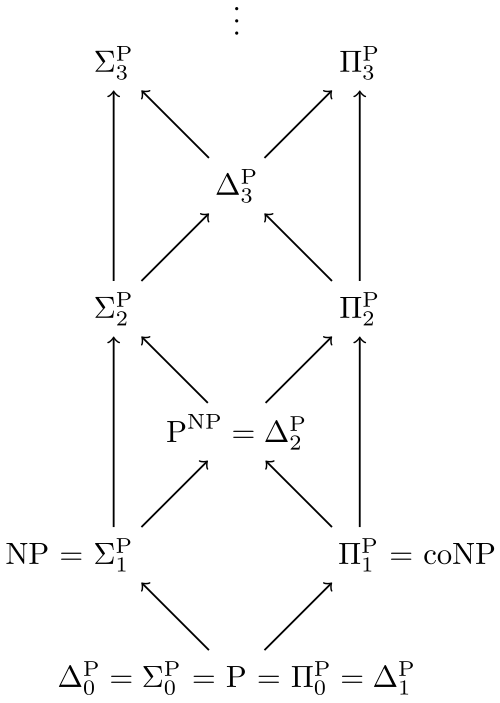
\includegraphics[width=5cm]{images/Polynomial_time_hierarchy.svg.png}};    
            \end{tikzpicture}
        \end{column}
    \end{columns}
\end{frame}

\begin{frame}{Fixed Points}
    \begin{itemize}
        \item $f:\cP(\cD)\rightarrow\cP(\cD)$
        \item \textbf{Monotone:} $X\subseteq Y$ implies $f(X)\subseteq f(Y)$
        \item \textbf{Inflationary:} $\forall X\in\cP(\cD): X\subseteq f(X)\subseteq f(f(X))\subseteq\ldots$
        \item \textbf{Fixed point:} $X\in\cP(D)$ is an FP of $f$, $f(X) = X$
    \end{itemize}
\end{frame}

\begin{frame}{Fixed Points}
    \begin{itemize}
        \item $X_0 = \emptyset$, $X_i = f^i(X_0)$
        \item If $f$ is monotone, $lfp(f) = \bigcup_{i\geq 0}X_i$
        \item What if not monotone?
        \begin{itemize}
            \item \textbf{Inflationary Fixed Point (IFP):} $ifp(f) = \bigcup_{i=0}^n (X_i\cup f(X_i))$
            \item \textbf{Partial Fixed Point (PFP):} $ pfp(f) = 
                                                                        \begin{cases} 
                                                                            X_n & X_n = X_{n+1} \\
                                                                            \emptyset & \forall n\leq 2^{|D|}:X_n \neq X_{n+1}
                                                                        \end{cases}
                                                        $
        \end{itemize}
        \item Extending logics using FP operators for higher definability
        \item \textbf{NOTE:} For MONOTONE functions: $lfp = ifp = pfp$
    \end{itemize}
\end{frame}

\begin{itemize}
    \item[] Below PH:
    \begin{block}{Immerman and Vardi}
    If query being done over \emph{ordered finite} structures then
    $$
    LFP\equiv\PTime
    $$    
    \end{block}

    \item[] Above PH:
    \begin{block}{$\PSPACE$ Characterisation}
        $$
        SO[TC]\equiv\PSPACE
        $$    
        \end{block}
\end{itemize}

\begin{frame}
    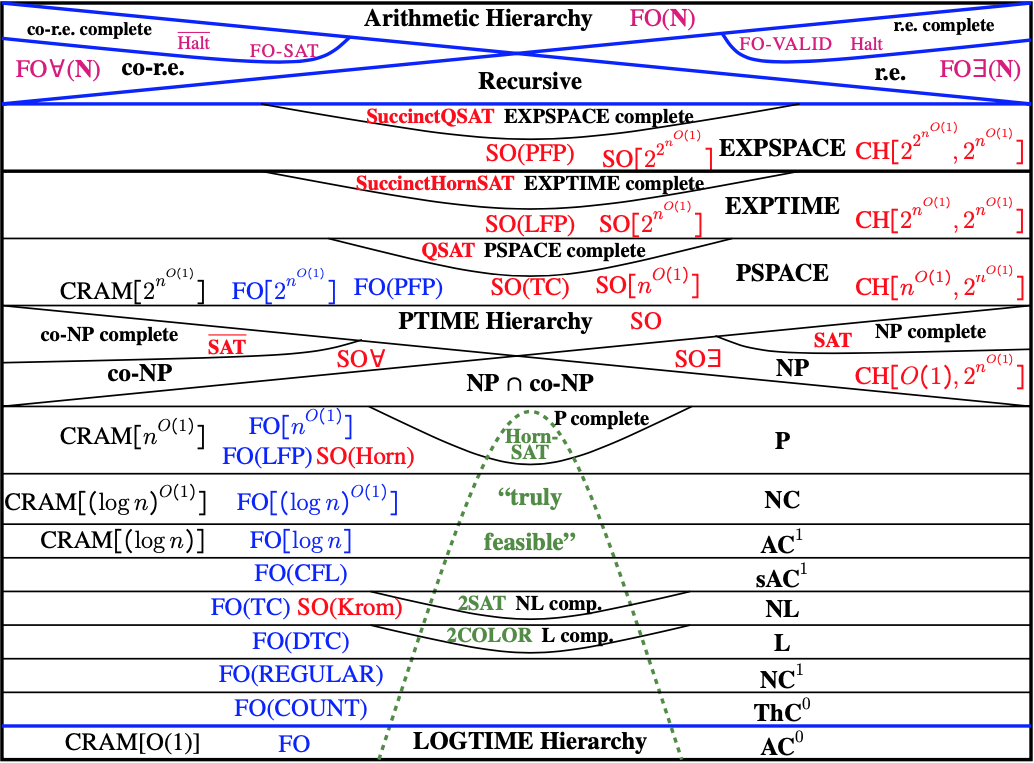
\includegraphics[scale = 0.3]{images/descriptiveWorld2023.jpg}
\end{frame}

\begin{frame}{Conclusion}
    \begin{itemize}
        \item \textbf{Other Aspects}: Proof Complexity
        \item \textbf{Open}: Exact Characterisations for $\PTime$
    \end{itemize}
\end{frame}
 
\end{document}

\begin{frame}{Thank You}
    \begin{figure}
        \centering
        
\includegraphics{images/question.jpg}
    \end{figure}
\end{frame}